% Copyright (C) 2022 - Joseph Muré

\documentclass{beamer}

%\setbeameroption{hide notes}
%\setbeameroption{show notes}
%\setbeameroption{show only notes}

% Copyright (C) 2012 - EDF R&D - Michael Baudin

% To highlight source code
\usepackage{listings}
\definecolor{darkgreen}{rgb}{0,0.5,0}
\definecolor{violet}{rgb}{0.5,0,1}

\usepackage{lmodern}% http://ctan.org/pkg/lm

\usetheme{Montpellier}
\setbeamertemplate{navigation symbols}{} % Remove navigation
\useoutertheme{infolines}

\usepackage[latin1]{inputenc}
\usepackage[T1]{fontenc}

%\usepackage[french]{babel}
%\uselanguage{French}
%\languagepath{French}

\def\bx{{\bf x}}
\def\RR{\mathbb{R}}

\newcommand{\pyvar}[1]{\texttt{#1}}

\def \ot {OpenTURNS}


\usepackage[
backend=biber,
style=alphabetic,
sorting=ynt
]{biblatex}

\usepackage{tikz}
\usetikzlibrary{positioning}

\renewcommand{\footnotesize}{\tiny}

\title[OpenTURNS]{Bayesian inference through MCMC sampling with OpenTURNS }

\author[Mur\'e]{
J. Mur\'e \inst{1} \and
M. Keller \inst{1}
}

\institute[EDF]{
\inst{1} EDF R\&D. 6, quai Watier, 78401, Chatou Cedex - France, joseph.mure@edf.fr \and %
}

\date[]{June 13th 2023, Journ\'ee AppliBUGS, Institut Henri Poincar\'e}

\definecolor{codegreen}{rgb}{0,0.6,0}
\definecolor{codegray}{rgb}{0.5,0.5,0.5}
\definecolor{codepurple}{rgb}{0.58,0,0.82}
\definecolor{backcolour}{rgb}{0.95,0.95,0.92}
\lstdefinestyle{mystyle}{
  escapechar={|},
  backgroundcolor=\color{backcolour},   commentstyle=\color{codegreen},
  keywordstyle=\color{magenta},
  numberstyle=\tiny\color{codegray},
  stringstyle=\color{codepurple},
  basicstyle=\ttfamily\tiny,
  breakatwhitespace=false,
  breaklines=true,
  captionpos=b,
  keepspaces=true,
  numbers=left,
  numbersep=5pt,
  showspaces=false,
  showstringspaces=false,
  showtabs=false,
  tabsize=1,
  numbers=none
}

\newcommand{\target}[1]{\textcolor{red}{#1}}
\newcommand{\proposal}[1]{\textcolor{blue}{#1}}
\newcommand{\support}[1]{\textcolor{orange}{#1}}
\newcommand{\prior}[1]{\textcolor{red}{#1}}
\newcommand{\likelihood}[1]{\textcolor{green}{#1}}
\newcommand{\observation}[1]{\textcolor{orange}{#1}}



\lstset{style=mystyle, language=python}

%%%%%%%%%%%%%%%%%%%%%%%%%%%%%%%%%%%%%%%%%%%%%%%%%%%%%%%%%%%%%%%%%%%%%%%%%%%%%

  \begin{document}

  \begin{frame}
    \titlepage

    \begin{columns}
      \column{0.45\textwidth}
      \centering
      
\includegraphics[height=0.15\textheight]{figures/logo-openturns.png}

      \column{0.45\textwidth}
      \centering
      
\includegraphics[height=0.15\textheight]{figures/edf.jpg}

     \end{columns}

    \end{frame}
%%%%%%%%%%%%%%%%%%%%%%%%%%%%%%%%%%%%%%%%%%%%%%%%%%%%%%%%%%%%%%%%%%%%%%%%%%%%%

%%%%%%%%%%%%%%%%%%%%%%%%%%%%%%%%%%%%%%%%%%%%%%%%%%%%%%%%%%%%%%%%%%%%%%%%%%%%%
\section{About OpenTURNS}
\begin{frame}
    \frametitle{OpenTURNS: \url{www.openturns.org}}


        \begin{center}
        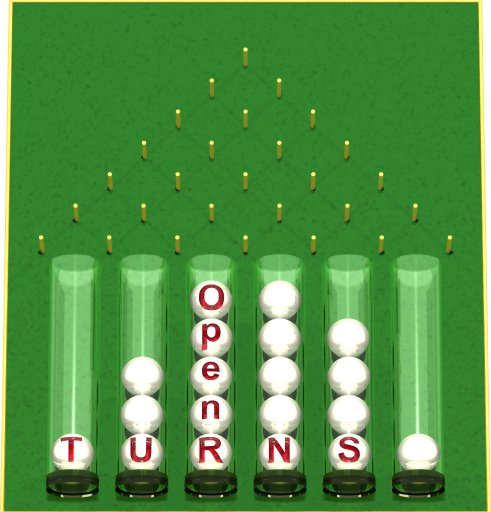
\includegraphics[width=0.3\textwidth]{figures/logo-ot.jpg}
        \end{center}

    \begin{itemize}
    \item Multivariate probabilistic modeling including dependence
    \item Numerical tools dedicated to the treatment of uncertainties
    \item Generic coupling to any type of physical model
    \item Open source, LGPL licensed, C++/Python library
    \end{itemize}


    \end{frame}

    \note{
    OpenTURNS is software for uncertainty quantification, uncertainty propagation,
    sensitivity analysis and metamodeling.

    It is available with the open source LGPL licence on Linux, Windows and macOS.

    In order to use OpenTURNS, you can use directly the C++ library, or
    program your Python scripts.
    }
    %%%%%%%%%%%%%%%%%%%%%%%%%%%%%%%%%%%%%%%%%%%%%%%%%%%%%%%%%%%%%%%%%%%%%%%%%%%%%

    \begin{frame}
    \frametitle{OpenTURNS: \url{www.openturns.org}}

    \begin{center}
       \begin{tabular}{ccccc}
       
\includegraphics[width=0.07\textwidth]{figures/logoEDF_Anne.png}&
       
\includegraphics[width=0.12\textwidth]{figures/LogoAirbus.png}&
       
\includegraphics[width=0.12\textwidth]{figures/logo_phimeca.png}&
       
\includegraphics[width=0.12\textwidth]{figures/logo_Imacs.png}
       
\includegraphics[width=0.30\textwidth]{figures/logo_ONERA.jpg}&
       \end{tabular}
    \end{center}

    \vspace*{0.05cm}
    \begin{itemize}
    \item Linux, Windows, macOS
    \item First release : 2007
    \item 5 full time developers
    \item Users $\approx 1000$, mainly in France
    (785 000 Total Conda downloads)
    \item Project size : 800  classes, more than 6000 services
    \end{itemize}


    \end{frame}

    %%%%%%%%%%%%%%%%%%%%%%%%%%%%%%%%%%%%%%%%%%%%%%%%%%%%%%%%%%%%%%%%%%%%%%%%%%%%%

    \begin{frame}[containsverbatim]
      \frametitle{OpenTURNS: content}

      \begin{scriptsize}

      \begin{minipage}[t]{0.33\textwidth}
      \begin{itemize}
      \item Data analysis
      \begin{itemize}
      \tiny
      \item Distribution fitting
      \item Statistical tests
      \item Estimate dependency and copulas
      \item Estimate stochastic processes
      \end{itemize}
      \end{itemize}
      \end{minipage}%
      \begin{minipage}[t]{0.33\textwidth}
      \begin{itemize}
      \item Probabilistic modeling
      \begin{itemize}
      \tiny
      \item Dependence modeling
      \item Univariate distributions
      \item Multivariate distrbutions
      \item Copulas
      \item Processes
      \item Covariance kernels
      \end{itemize}
      \end{itemize}
      \end{minipage}%
      \begin{minipage}[t]{0.33\textwidth}
      \begin{itemize}
      \item Surrogate models
      \begin{itemize}
      \tiny
      \item Linear regression
      \item Polynomial chaos expansion
      \item Gaussian  process regression
      \item Spectral methods
      \item Low rank tensors
      \item Fields metamodel
      \end{itemize}
      \end{itemize}
      \end{minipage}

      \vspace{20pt}

      \begin{minipage}[t]{0.33\textwidth}
      \begin{itemize}
      \item Reliability, sensitivity
      \begin{itemize}
      \tiny
      \item Sampling methods
      \item Approximation methods
      \item Sensitivity analysis
      \item Design of experiments
      \end{itemize}
      \end{itemize}
      \end{minipage}%
      \begin{minipage}[t]{0.33\textwidth}
      \begin{itemize}
      \item Calibration
      \begin{itemize}
      \tiny
      \item Least squares calibration
      \item Gaussian calibration
      \item Bayesian calibration
      \end{itemize}
      \end{itemize}
      \end{minipage}%
      \begin{minipage}[t]{0.33\textwidth}
      \begin{itemize}
      \item Numerical methods
      \begin{itemize}
      \tiny
      \item Optimization
      \item Integration
      \item Least squares
      \item Meshing
      \item Coupling with external codes
      \end{itemize}
      \end{itemize}
      \end{minipage}
      \end{scriptsize}

      \begin{tabular}{@{}c@{}c@{}c@{}c@{}c@{}}
      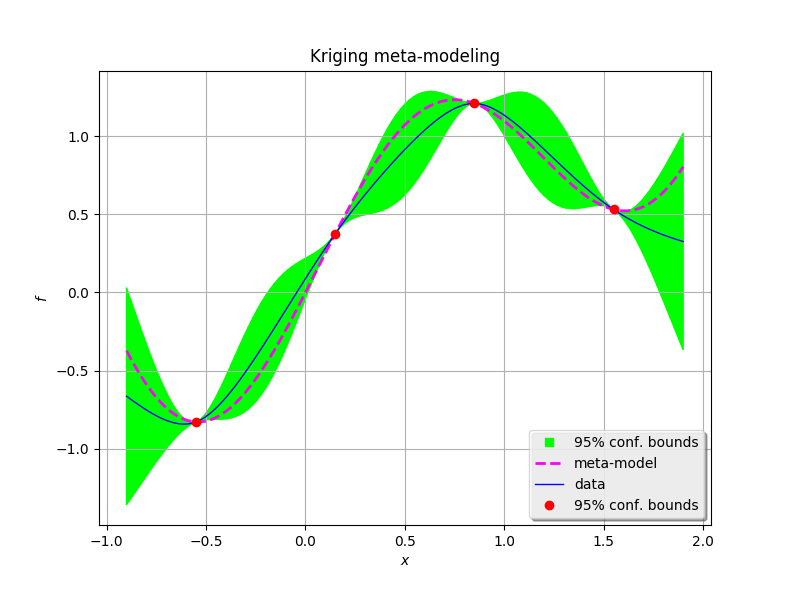
\includegraphics[width=0.2\textwidth]{figures/plot_kriging.png}&
      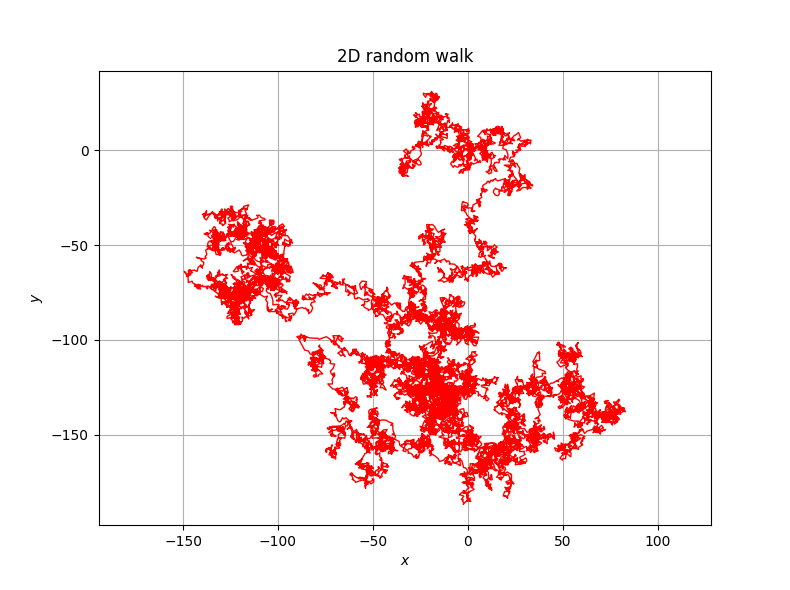
\includegraphics[width=0.2\textwidth]{figures/plot_random_walk.png}&
      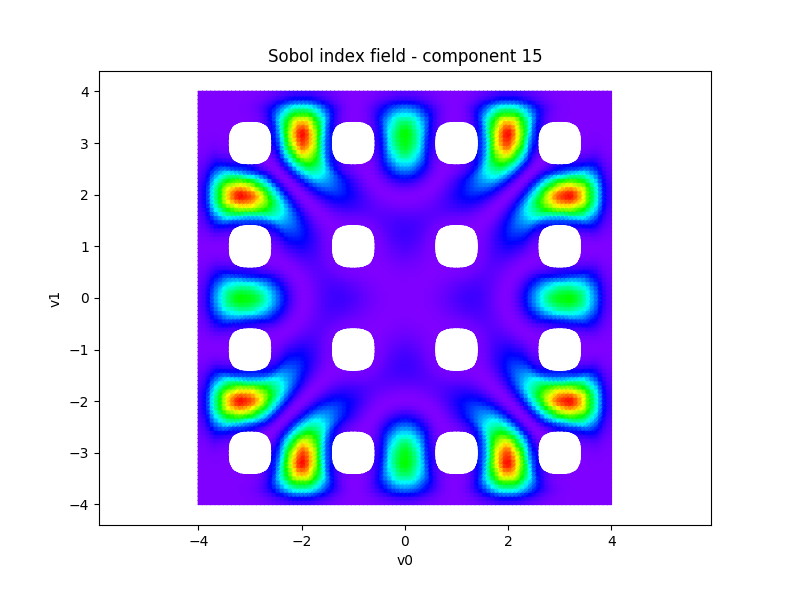
\includegraphics[width=0.2\textwidth]{figures/plot_sobol_field.png}&
      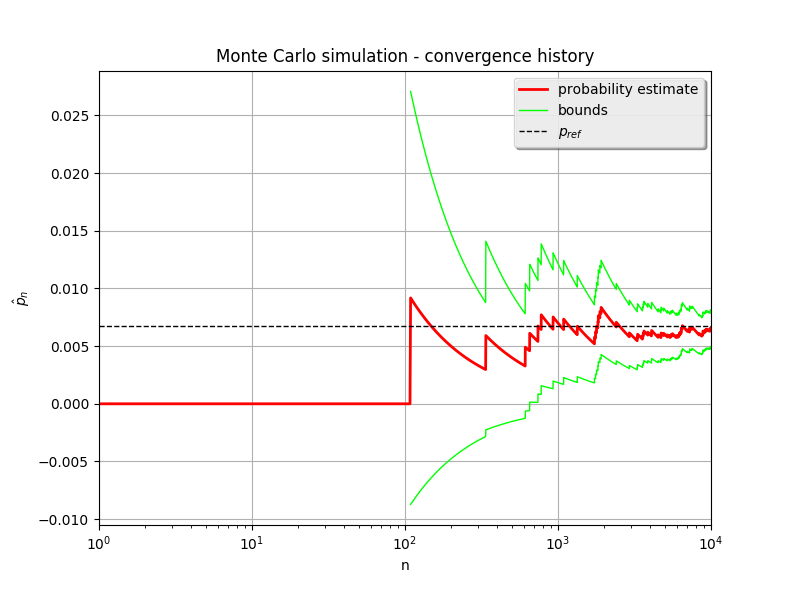
\includegraphics[width=0.2\textwidth]{figures/plot_monte_carlo.png}&
      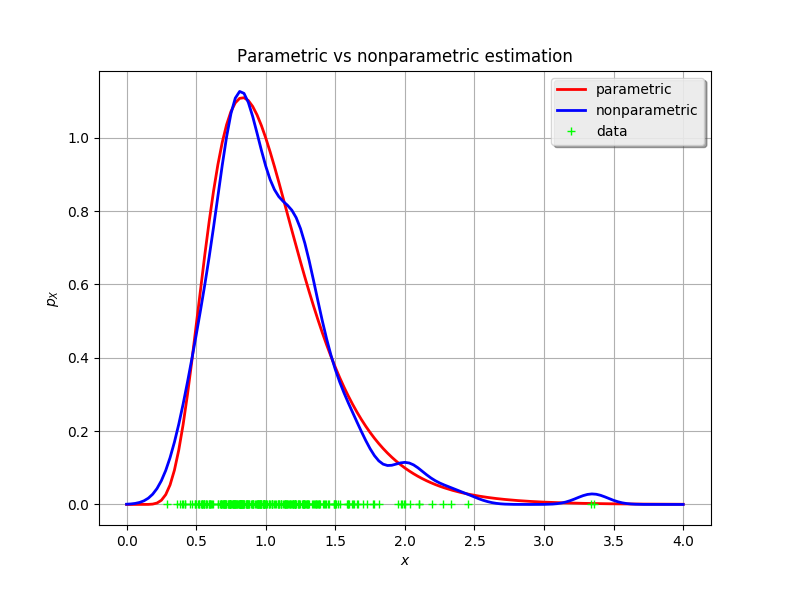
\includegraphics[width=0.2\textwidth]{figures/plot_distribution_fitting.png}
      \end{tabular}
    \end{frame}


    %%%%%%%%%%%%%%%%%%%%%%%%%%%%%%%%%%%%%%%%%%%%%%%%%%%%%%%%%%%%%%%%%%%%%%%%%%%%%

    \begin{frame}[containsverbatim]
      \frametitle{OpenTURNS: documentation}

      \small{

      \begin{columns}
          \column{0.5\textwidth}

          \begin{center}
          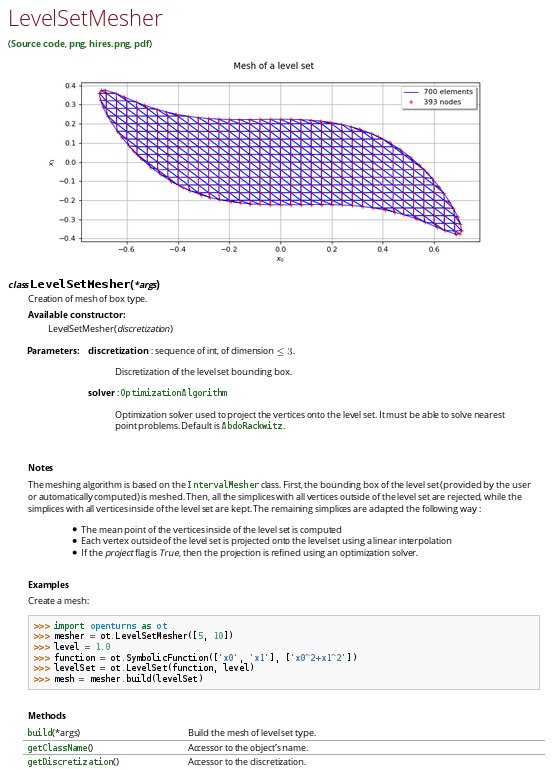
\includegraphics[width=0.8\textwidth]{figures/exClasses.png}
          \end{center}

          \column{0.5\textwidth}

        \begin{itemize}
        \item \underline{Content}:
        \begin{itemize}
        \item Programming interface (API)
        \item Examples
        \item Theory
        \end{itemize}
        \item \emph{All} classes and methods
        are documented, partly automatically.
        \item Examples are automatically tested at \emph{each} update
        of the code and outputs are checked.
        \end{itemize}

      \end{columns}

      }
    \end{frame}

    %%%%%%%%%%%%%%%%%%%%%%%%%%%%%%%%%%%%%%%%%%%%%%%%%%%%%%%%%%%%%%%%%%%%%%%%%%%%%

    \begin{frame}[containsverbatim]
      \frametitle{Coupling OpenTURNS with computer codes}

      \small

      OpenTURNS provides a text file exchange based interface in order to perform analyses on complex computer codes

      \vspace{10pt}

      \begin{columns}
          \column{0.6\textwidth}

      \centering

      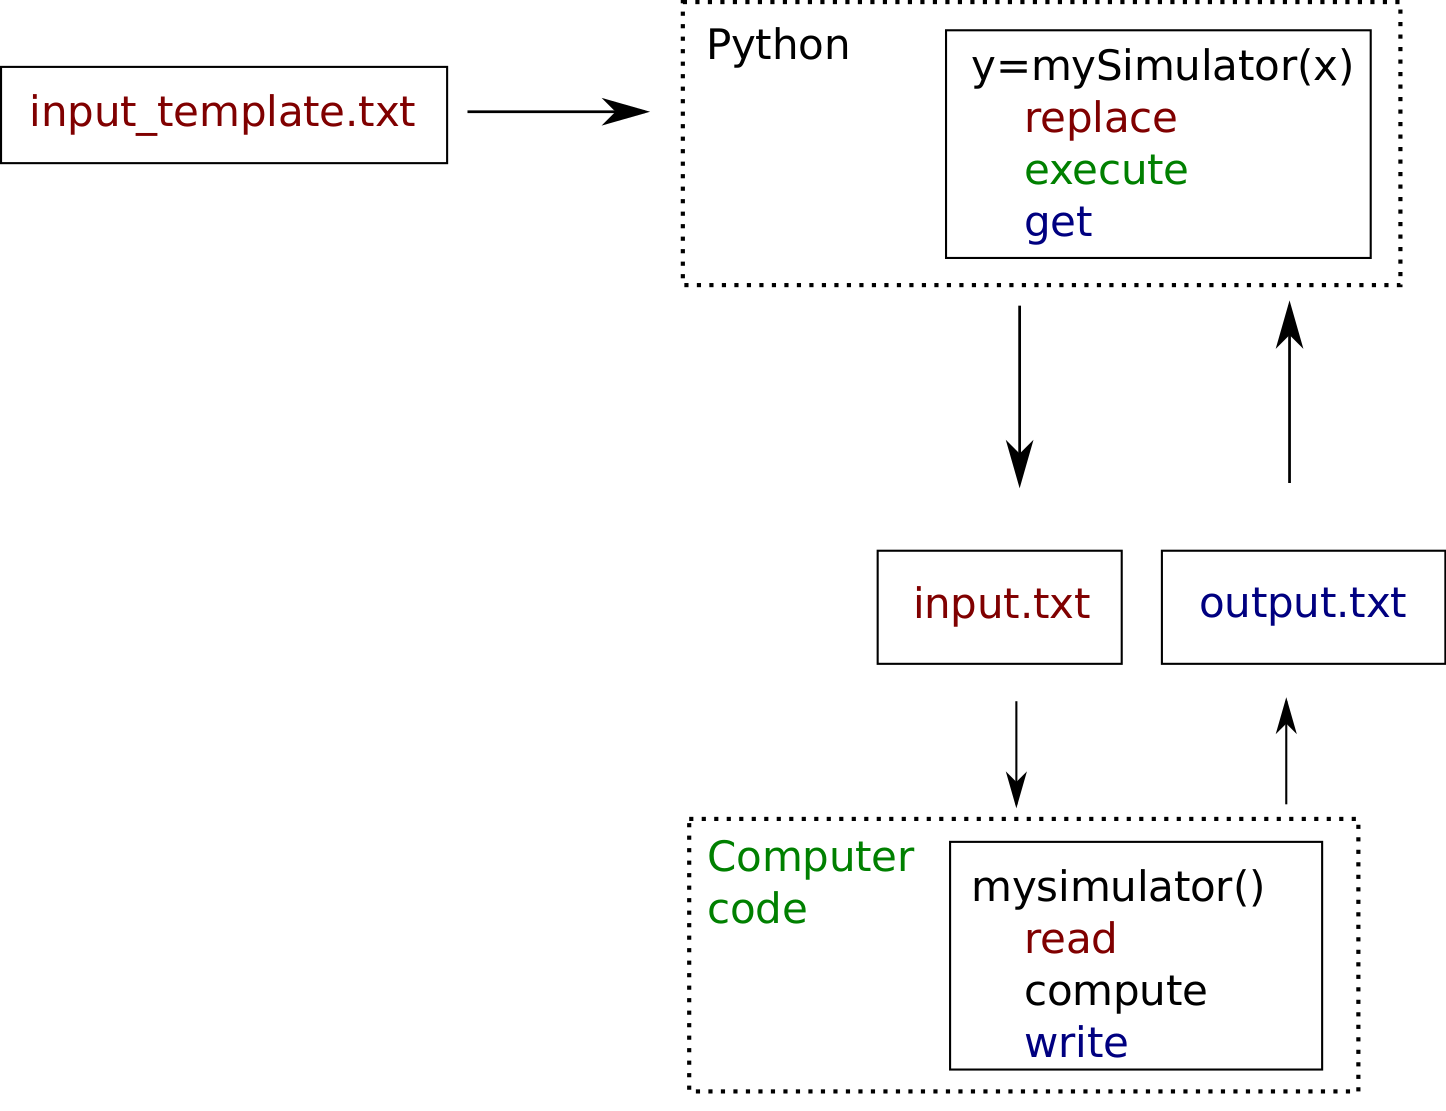
\includegraphics[width=1.\textwidth]{figures/Coupling.png}

          \column{0.4\textwidth}

      \begin{itemize}
      \item Replaces the need for input/output text parsers
      \item Wraps a simulation code under the form of a standard python function
      \item Allows to interface OpenTURNS with a cluster
      \item \href{https://openturns.github.io/otwrapy/master/index.html}{otwrapy}: interfacing tool to allow easy parallelization
      \end{itemize}

      \end{columns}

    \end{frame}

\begin{frame}
    \frametitle{Contents}
    \tableofcontents
    \end{frame}

%%%%%%%%%%%%%%%%%%%%%%%%%%%%%%%%%%%%%%%%%%%%%%%%%%%%%%%%%%%%%%%%%%%%%%%%%%%%%








%%%%%%%%%%%%%%%%%%%%%%%%%%%%%%%%%%%%%%%%%%%%%%%%%%%%%%%%%%%%%%%%%%%%%%%%%%%%%
\section{The Metropolis-Hastings algorithm}
\begin{frame}[containsverbatim]
    \frametitle{OpenTURNS: Metropolis-Hastings}
    \small
    We want to sample from the distribution $\target{\pi}$ of a random variables $X$.
    Here is one step of the algorithm, starting from the point $x$:

    \begin{enumerate}
    \item Simulate a candidate $x' \sim \proposal{q( \cdot | x)}$ for some conditional distribution $q$.
    \item Compute
    $
    \alpha(x' | x,y,z) = \min \left\{ \frac{\target{\pi(x')} \, \proposal{q(x | x')}}{\target{\pi(x)} \proposal{q(x' | x)}} , 1 \right\}.
    $
    \item Simulate $u \sim \mathcal{U}(0,1)$. If $u \leqslant \alpha(x'| x)$,
    then the next state is $x'$, otherwise it is $x$.
    \end{enumerate}

    Throughout the presentation, our code is prefaced by:

    \begin{lstlisting}
    import openturns as ot
    import math as m
    import numpy as np
    \end{lstlisting}
\end{frame}

%%%%%%%%%%%%%%%%%%%%%%%%%%%%%%%%%%%%%%%%%%%%%%%%%%%%%%%%%%%%%%%%%%%%%%%%%%%%%
\section{Random walk Metropolis-Hastings}
\begin{frame}[containsverbatim]{Random walk Metropolis Hastings}

    When $q(\cdot | x) = x + \proposal{\mu}$, where $\proposal{\mu}$ is a distribution that does not depend on $x$,
    the  algorithm is called ``Random walk Metropolis-Hastings'' and $\proposal{}\mu$ is called the ``proposal distribution''.


    \begin{block}{Sample from a nonstandard distribution\footnote{Marin , J.M. and Robert, C.P. (2007). Bayesian Core: A Practical Approach to Computational Bayesian Statistics. \emph{Springer-Verlag}, New York}}
        \begin{columns}
            \begin{column}{0.4\textwidth}
                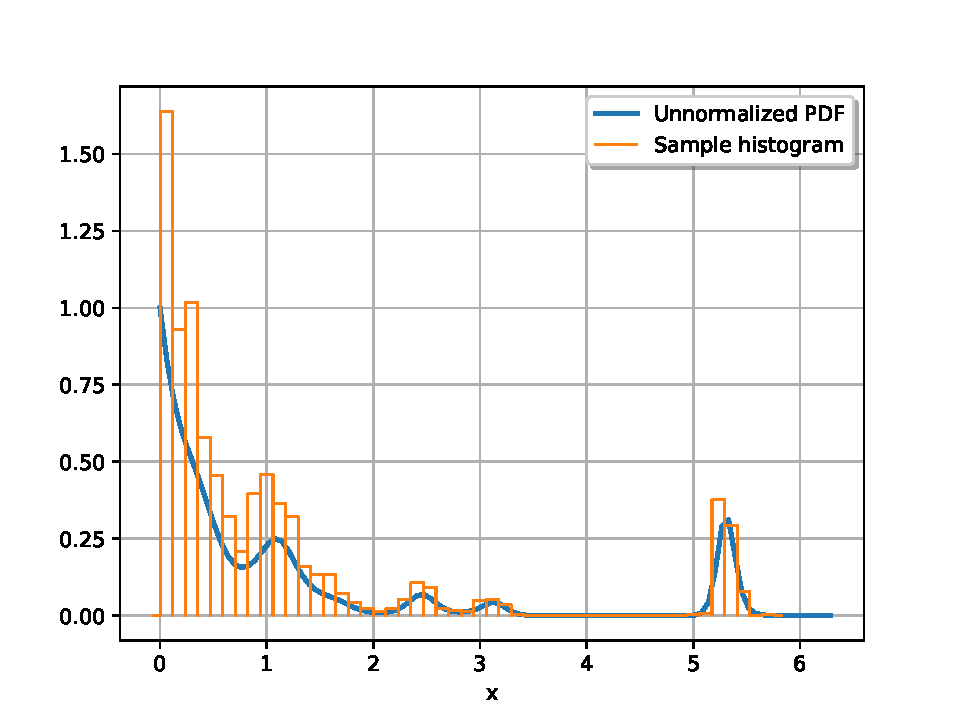
\includegraphics[width=\textwidth]{figures/ChristianRobert_tough_density}
            \end{column}
            \begin{column}{0.6\textwidth}
                \vspace{-0.5cm}
                \begin{align*}
                    & \pi(x) \\ \propto & \frac{1}{2} \target{(2 + \sin(x)^2)} \\
                    & \target{\exp \left[- \left(2 + \cos(3x)^3 + \sin(2x)^3 \right) x \right]} \\
                    & \support{\mathbf{1}_{[0, 2 \pi]}(x)}
                \end{align*}
            \end{column}
        \end{columns}


\vspace{-0.4cm}
\begin{lstlisting}
|\target{logdensity}| = ot.|Symbolic\target{Function}|('x','log(2+sin(x)^2) - (2+cos(3*x)^3+sin(2*x)^3) * x')
|\support{support = ot.Interval([0.0], [2.0 * m.pi])}|
|\proposal{proposal = ot.Normal(0.0, 2.0)}| # mu
initialState = [3.0]
sampler = ot.RandomWalkMetropolisHastings(|\target{logdensity}|, |\support{support}|, initialState, |\proposal{proposal}|)
x = sampler.getSample(10000)
\end{lstlisting}
    \end{block}
\end{frame}

%%%%%%%%%%%%%%%%%%%%%%%%%%%%%%%%%%%%%%%%%%%%%%%%%%%%%%%%%%%%%%%%%%%%%%%%%%%%%

\begin{frame}[containsverbatim]{2D Random walk Metropolis Hastings}

    \begin{block}{Sample from a 2D nonstandard distribution}
        \begin{columns}
            \begin{column}{0.4\textwidth}
                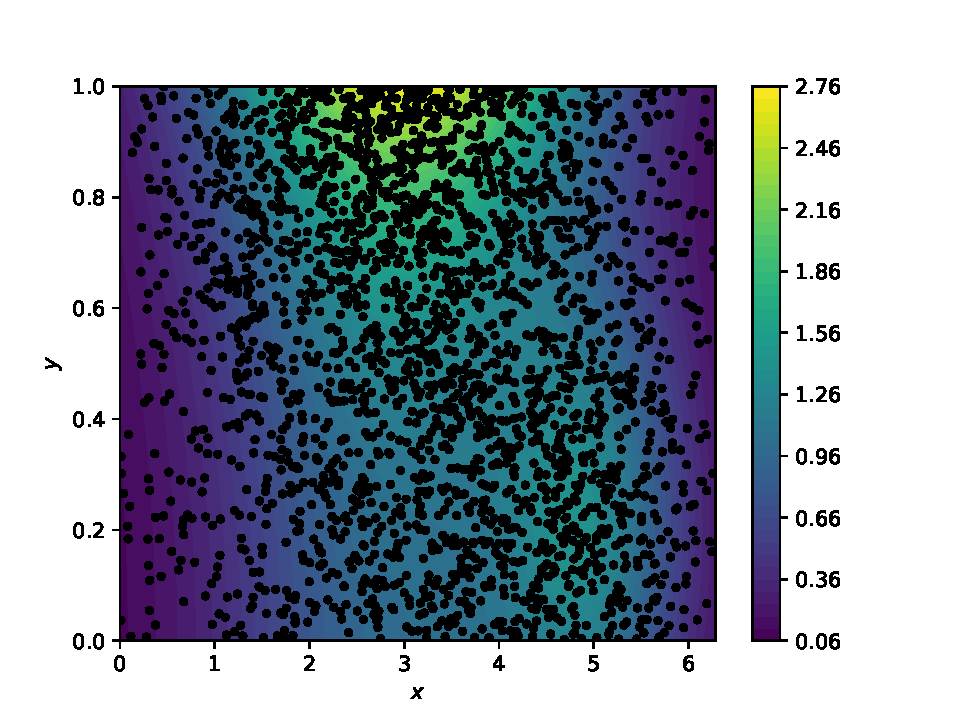
\includegraphics[width=\textwidth]{figures/2d}
            \end{column}
            \begin{column}{0.6\textwidth}
                \vspace{-0.5cm}
                \begin{align*}
                    & \pi(x) \\ \propto & \target{\left( \exp\left[-\frac{1}{4} (x-3)^2 + y^2\right] \right.}\\
                    & \target{ \left. + \exp\left[-(x-5)^2 - 5 \left(y-\frac{1}{5} \right)^2 \right] \right) }\\
                    & \; \support{\mathbf{1}_{[0, 2 \pi]}(x)} \support{\mathbf{1}_{[0, 1]}(y)}
                \end{align*}
            \end{column}
        \end{columns}



\begin{lstlisting}
|\target{logdensity}| = ot.|Symbolic\target{Function}|(
    ["x", "y"], ["log(exp(-0.25 * (x-3)^2 + y^2) + exp(-(x-5)^2 - 5 * (y-0.2)^2))"]
)
|\support{support = ot.Interval([0.0, 0.0], [2.0 * m.pi, 1.0])}|
|\proposal{proposal = ot.Normal([0.0] * 2, [1.0, 0.2])}|
initialState = [3.0, 0.8]
sampler = ot.RandomWalkMetropolisHastings(|\target{logdensity}|, |\support{support}|, initialState, |\proposal{proposal}|)
x = sampler.getSample(50000)
\end{lstlisting}
    \end{block}
\end{frame}

%%%%%%%%%%%%%%%%%%%%%%%%%%%%%%%%%%%%%%%%%%%%%%%%%%%%%%%%%%%%%%%%%%%%%%%%%%%%%

\begin{frame}[containsverbatim]{2D Random walk Metropolis Hastings in a Bayesian setting}

    \begin{block}{Posterior distribution of the parameters of a Weibull model}
        \begin{columns}
            \begin{column}{0.4\textwidth}
                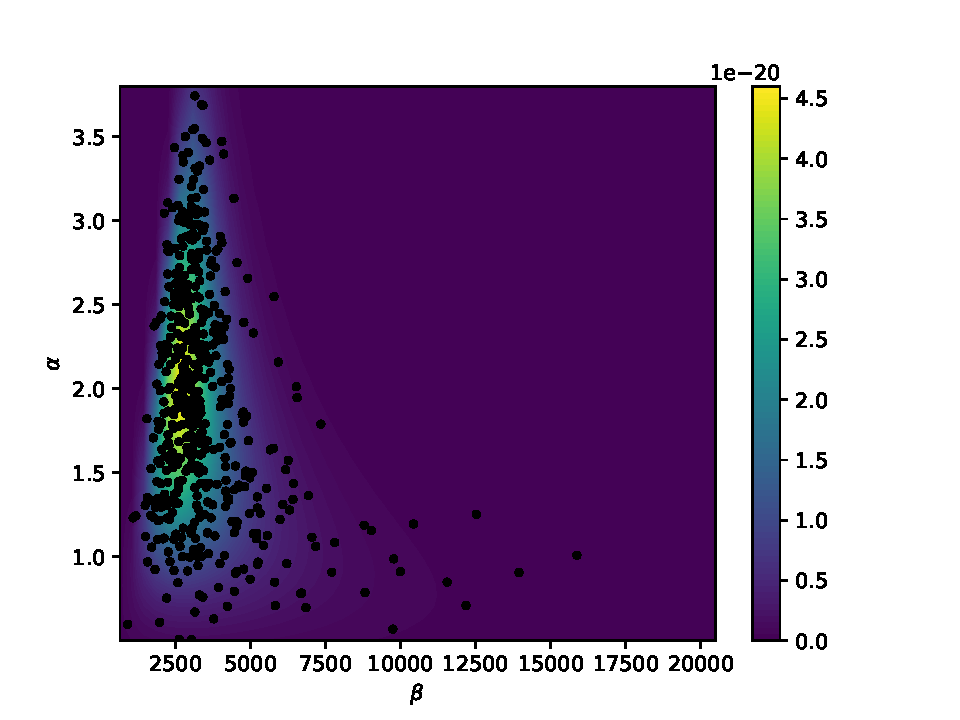
\includegraphics[width=\textwidth]{figures/fiabilite}
            \end{column}
            \begin{column}{0.6\textwidth}
                \vspace{-0.5cm}
                \begin{align*}
                    \beta &\sim \prior{\Gamma(k=2, \lambda=2\cdot 10^{-4})} \\
                    \alpha &\sim \prior{\mathcal{U}(0.5, 3.8)} \\
                    \observation{T} | \beta, \alpha &\sim \likelihood{\mathcal{W}}(\beta, \alpha, 0) \\
                    F_{\mathcal{W}}(t) &= 1 - \exp \left[ - \left( \frac{t - 0}{\beta}\right)^\alpha\right]
                \end{align*}
            \end{column}
        \end{columns}



\begin{lstlisting}
alpha_min, alpha_max, a_beta, b_beta = 0.5, 3.8, 2.0, 2.0e-4
priorMarginals = [ot.|\prior{Gamma}|(a_beta, b_beta), ot.|\prior{Uniform}|(alpha_min, alpha_max)]
|\target{prior}| = ot.ComposedDistribution(priorMarginals)
|\proposal{proposal}| = ot.Normal([0.0]*2, [0.1*m.sqrt(a_beta/b_beta**2), 0.1*(alpha_max-alpha_min)])
initialState = [a_beta / b_beta, 0.5 * (alpha_max - alpha_min)]
sampler = ot.RandomWalkMetropolisHastings(|\target{prior}|, initialState, |\proposal{proposal}|)

|\likelihood{conditional} = ot.\likelihood{WeibullMin()}|
|\observation{Tobs}| = [[4380], [1791], [1611], [1291]]

# WeibullMin expects beta, alpha, and localization, but the prior is only on beta, alpha
linkFunction = ot.SymbolicFunction(["beta", "alpha"], ["beta", "alpha", "0"])
sampler.setLikelihood(|\likelihood{conditional}|, |\observation{Tobs}|, linkFunction)
sample = sampler.getSample(100000)
\end{lstlisting}
\end{block}
\end{frame}


%%%%%%%%%%%%%%%%%%%%%%%%%%%%%%%%%%%%%%%%%%%%%%%%%%%%%%%%%%%%%%%%%%%%%%%%%%%%%
\section{The Gibbs algorithm}
\begin{frame}[containsverbatim]{A flood model}

%    \begin{block}{Model description}
        \begin{columns}
            \begin{column}{0.35\textwidth}
                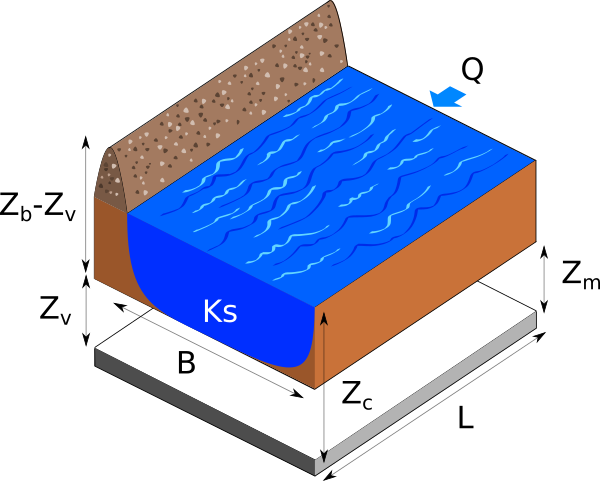
\includegraphics[width=\textwidth]{figures/flooding_section}
                \begin{align*}
                    &\forall \, 1 \leq i  \leq 8, \observation{H^{(i)}} \sim \\
                      \likelihood{\mathcal{N}} &\left(G(\observation{Q^{(i)}}, K_s, Z_v, Z_m), \frac{1}{2}\right)
                \end{align*}
            \end{column}
            \begin{column}{0.65\textwidth}
                \begin{lstlisting}
|\observation{Qobs} = [[2097], [1448], [1516], [2173], [387], [3016], [651], [541]]|
|\observation{Hobs} = [[3.4], [2.5], [2.7], [3.5], [1.0], [4.2], [1.6], [1.6]]|

def flooding(X):
    L = 5.0e3
    B = 300.0
    Q, K_s, Z_v, Z_m = X
    alpha = (Z_m - Z_v) / L
    if alpha < 0.0 or K_s <= 0.0:
        H = np.inf
    else:
        H = (Q / (K_s * B * np.sqrt(alpha))) ** (3.0 / 5.0)
    return [H, 0.5]

functionG = ot.PythonFunction(4, 2, flooding)

# Q (input #0) is not calibrated
linkFunction = ot.ParametricFunction(functionG, |\observation{[0]}|, |[100]|)
                \end{lstlisting}
            \end{column}
        \end{columns}


%\end{block}

%\begin{block}{Prior description}
    \begin{columns}
        \begin{column}{0.36\textwidth}
            \begin{align*}
                \prior{K_s} \, &\prior{\sim \mathcal{N}(20, 5)} \\
                \prior{Z_v} \, &\prior{\sim \mathcal{N}(49, 1)} \\
                \prior{Z_m} \, &\prior{\sim \mathcal{N}(51, 1)}
            \end{align*}
        \end{column}
        \begin{column}{0.64\textwidth}
            \begin{lstlisting}
|\likelihood{conditional}| = |ot.\likelihood{Normal()}|

parameterPriorMean = [20.0, 49.0, 51.0]
parameterPriorSigma = [5.0, 1.0, 1.0]
|\prior{prior}| = |ot.\prior{Normal(parameterPriorMean, parameterPriorSigma)}|

initialState = parameterPriorMean
            \end{lstlisting}
        \end{column}
    \end{columns}

%\end{block}
\end{frame}

%%%%%%%%%%%%%%%%%%%%%%%%%%%%%%%%%%%%%%%%%%%%%%%%%%%%%%%%%%%%%%%%%%%%%%%%%%%%%


\begin{frame}[containsverbatim]
    \frametitle{Single component Random Walk Metropolis-Hastings}
    \centering
    \vspace{0.5cm}
    
\begin{tikzpicture}[
    squarednode/.style={rectangle, draw=green!60, fill=green!5, very thick, minimum size=5mm},
    ]
    %Nodes
    \node[squarednode]      (mhx)                              {\texttt{mh\_Ks}};
    \node[squarednode]      (mhy)       [right=of mhx] {{\texttt{mh\_Zv}}};
    \node[squarednode]      (mhz)       [right=of mhy] {{\texttt{mh\_Zm}}};

    %Lines
    \draw[->] (mhx.east) -- (mhy.west);
    \draw[->] (mhy.east) -- (mhz.west);
    \draw[->] (mhz.east) to [out=340,in=200,looseness=1] (mhx.west);
    \end{tikzpicture}

    \begin{lstlisting}
mh_coll = [
  ot.RandomWalkMetropolisHastings(|\prior{prior}|, initialState, |ot.\proposal{Uniform(-5.0, 5.0)}|, [0]),
  ot.RandomWalkMetropolisHastings(|\prior{prior}|, initialState, |ot.\proposal{Uniform(-1.0, 1.0)}|, [1]),
  ot.RandomWalkMetropolisHastings(|\prior{prior}|, initialState, |ot.\proposal{Uniform(-1.0, 1.0)}|, [2]),
]

for mh in mh_coll:
    mh.setLikelihood(|\likelihood{conditional}|, |\observation{Hobs}|, linkFunction, |\observation{Qobs}|)

sampler = ot.Gibbs(mh_coll) # NB: the order can be made random: cf. setUpdatingMethod
sample = sampler.getSample(10000)
    \end{lstlisting}

    \begin{figure}
    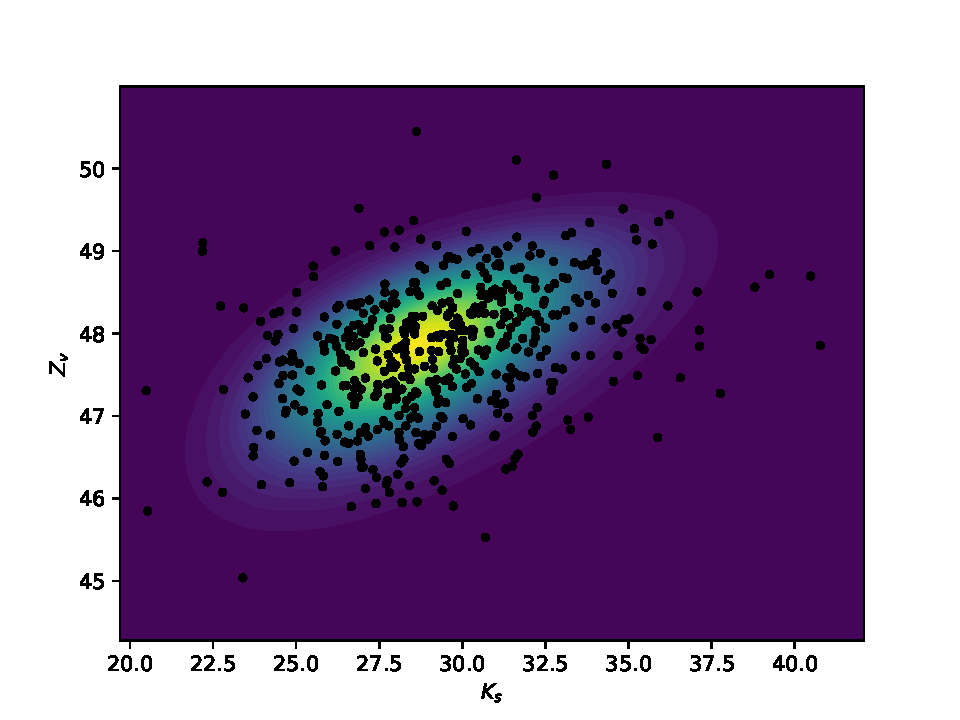
\includegraphics[width=0.32\textwidth]{figures/crue_gibbs_scmh_Z_v_K_s.pdf}
    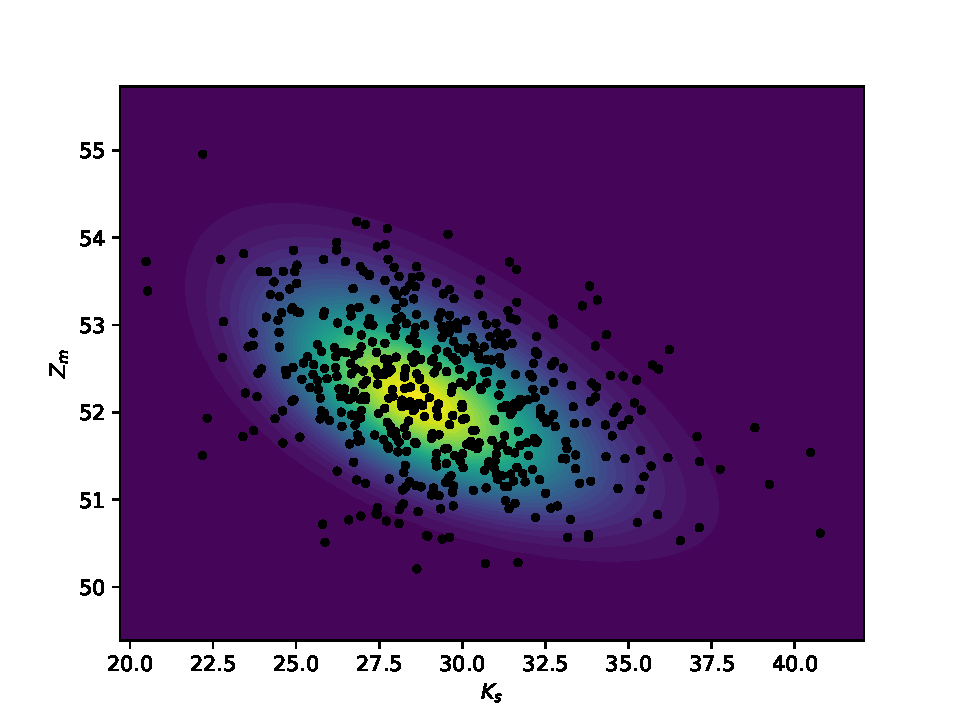
\includegraphics[width=0.32\textwidth]{figures/crue_gibbs_scmh_Z_m_K_s.pdf}
    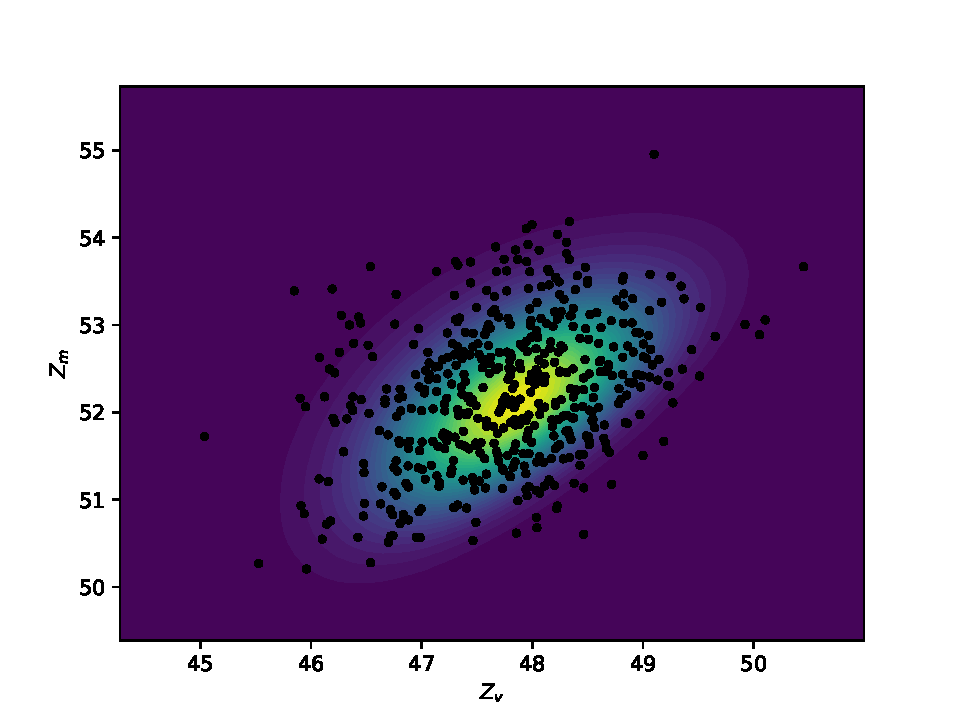
\includegraphics[width=0.32\textwidth]{figures/crue_gibbs_scmh_Z_m_Z_v.pdf}
    \end{figure}
\end{frame}

%%%%%%%%%%%%%%%%%%%%%%%%%%%%%%%%%%%%%%%%%%%%%%%%%%%%%%%%%%%%%%%%%%%%%%%%%%%%%

\begin{frame}[containsverbatim]
    \frametitle{Blocks of components can be considered}
    \medskip
    \centering
    \vspace{0.25cm}
    
\begin{tikzpicture}[
    squarednode/.style={rectangle, draw=green!60, fill=green!5, very thick, minimum size=5mm},
    ]
    %Nodes
    \node[squarednode]      (mhxy)                     {\texttt{mh\_Ks}};
    \node[squarednode]      (mhz)       [right=of mhxy] {\texttt{mh\_Zv\_Zm}};

    %Lines
    \draw[->] (mhxy.east) -- (mhz.west);
    \draw[->] (mhz.east) to [out=340,in=200,looseness=1.5] (mhxy.west);

    \end{tikzpicture}

    \begin{lstlisting}
mh_coll = [
  ot.RandomWalkMetropolisHastings(|\prior{prior}|, initialState, |ot.\proposal{Uniform(-5.0, 5.0)}|, [0]),
  ot.RandomWalkMetropolisHastings(|\prior{prior}|,
                                  initialState,
                                  ot.|\proposal{ComposedDistribution([ot.Uniform(-1.0,1.0)]*2)}|,
                                  [1, 2])
]
for mh in mh_coll:
    mh.setLikelihood(|\likelihood{conditional}|, |\observation{Hobs}|, linkFunction, |\observation{Qobs}|)
sampler = ot.Gibbs(mh_coll) # NB: the order can be made random: cf. setUpdatingMethod
sample = sampler.getSample(10000)
            \end{lstlisting}

            \begin{figure}
            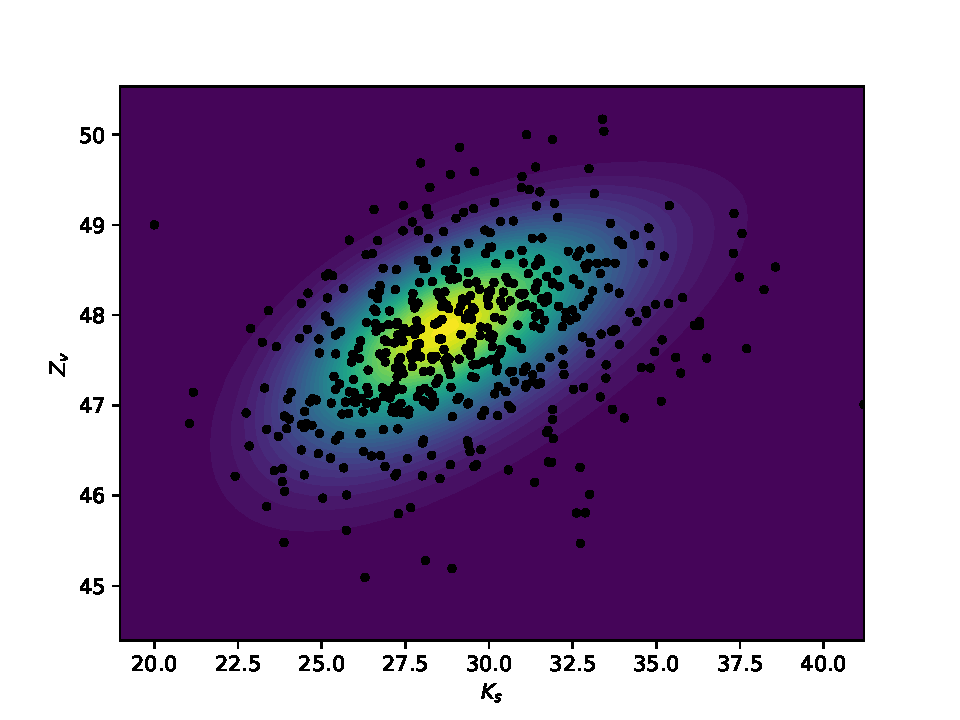
\includegraphics[width=0.32\textwidth]{figures/crue_gibbs_blocs_Z_v_K_s.pdf}
            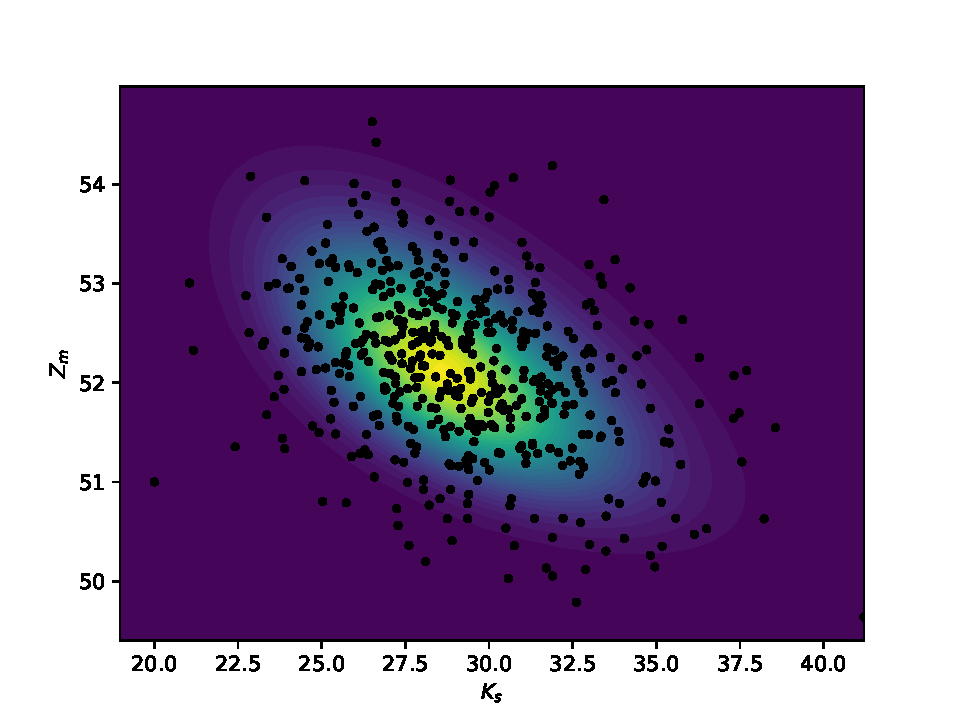
\includegraphics[width=0.32\textwidth]{figures/crue_gibbs_blocs_Z_m_K_s.pdf}
            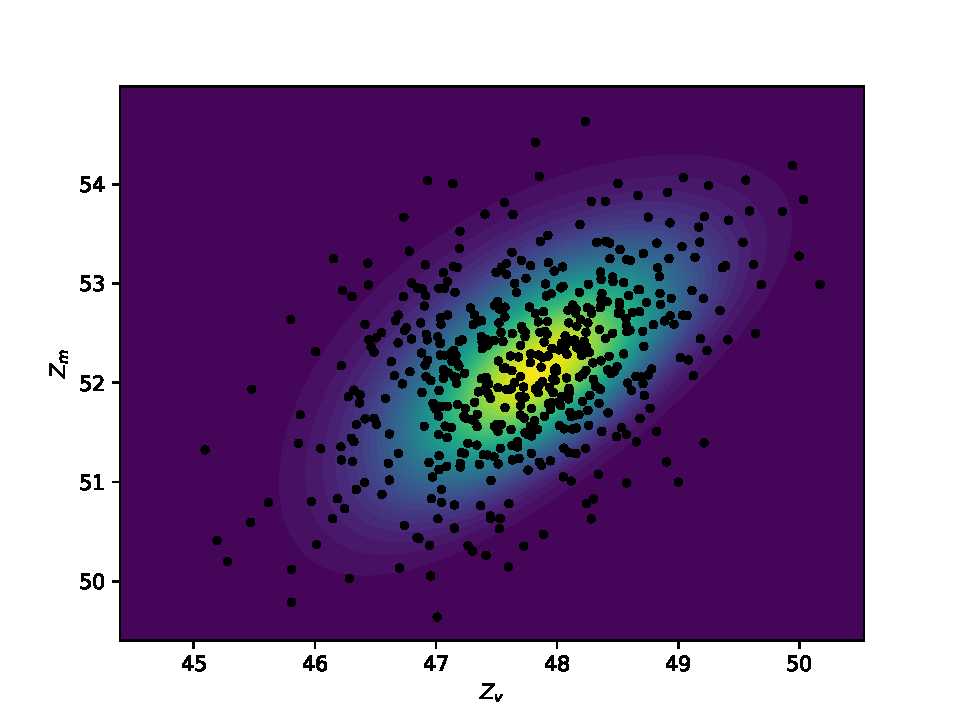
\includegraphics[width=0.32\textwidth]{figures/crue_gibbs_blocs_Z_m_Z_v.pdf}
            \end{figure}
\end{frame}

%%%%%%%%%%%%%%%%%%%%%%%%%%%%%%%%%%%%%%%%%%%%%%%%%%%%%%%%%%%%%%%%%%%%%%%%%%%%%
\section{Independent Metropolis-Hastings}
\begin{frame}[containsverbatim]
    \frametitle{Independent Metropolis-Hastings: $q(\cdot | x) = \mu$}
\begin{columns}
    \begin{column}{0.4\textwidth}
        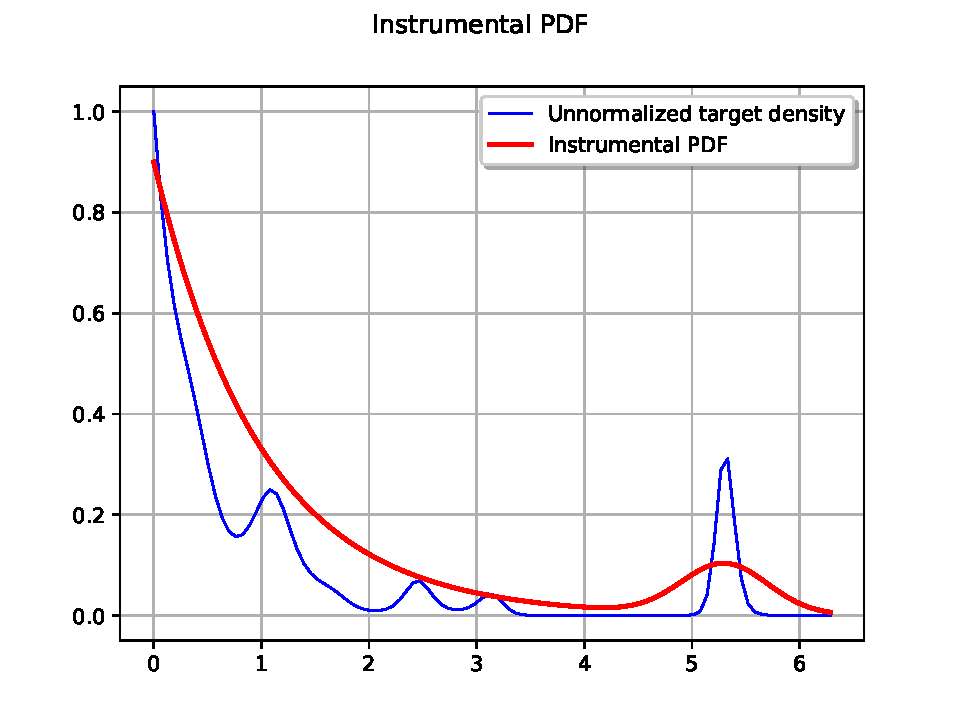
\includegraphics[width=\textwidth]{figures/instrumental}
    \end{column}
    \begin{column}{0.6\textwidth}
        \begin{lstlisting}
|\target{logdensity}| = ot.|Symbolic\target{Function}|('x','...') # replace ...
|\support{support = ot.Interval([0.0], [2.0 * m.pi])}|
initialState = [3.0] # unimportant for independent MH

exp = ot.Exponential(1.0)
unif = ot.Normal(5.3, 0.4)
|\proposal{instrumental}| = |ot.\proposal{Mixture([exp, unif], [0.9, 0.1])}|

independentMH = ot.IndependentMetropolisHastings(
  |\target{logdensity}|, |\support{support}|, initialState, |\proposal{instrumental}|
)
x = independentMH.getSample(10000)
        \end{lstlisting}
    \end{column}
\end{columns}

\begin{columns}
    \begin{column}{0.46\textwidth}
        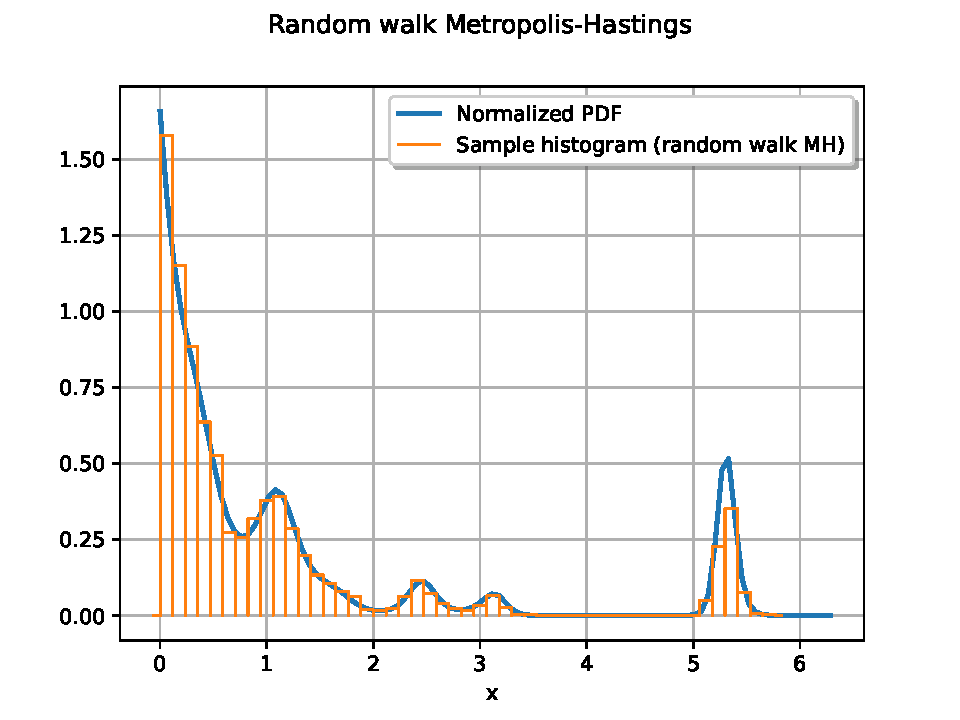
\includegraphics[width=\textwidth]{figures/randomwalkMH}
    \end{column}
    \begin{column}{0.46\textwidth}
        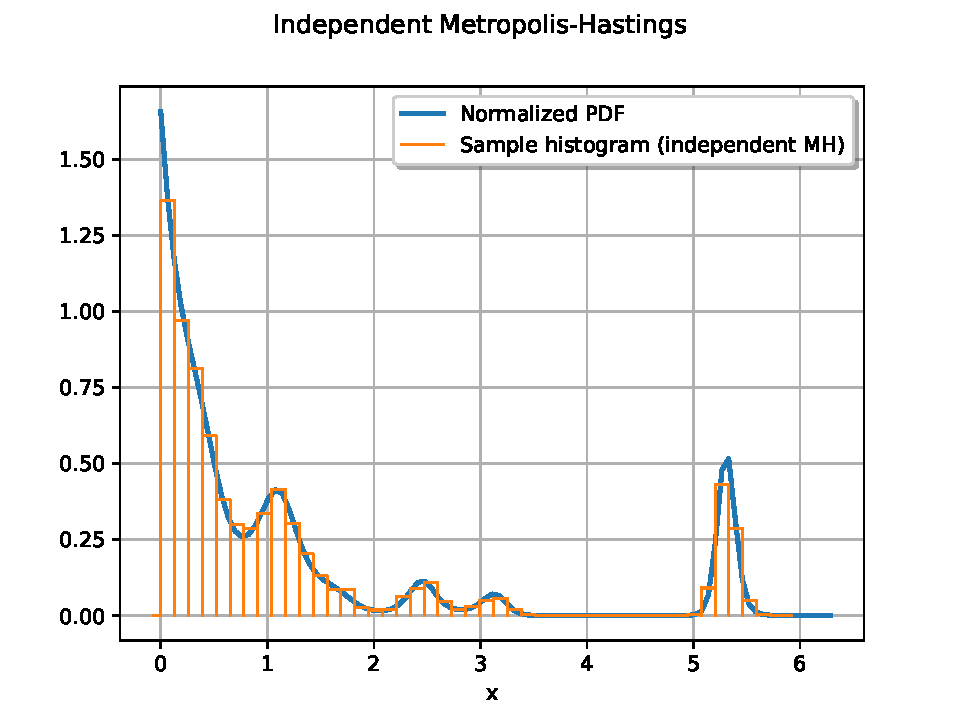
\includegraphics[width=\textwidth]{figures/independentMH}
    \end{column}
\end{columns}
\end{frame}

%%%%%%%%%%%%%%%%%%%%%%%%%%%%%%%%%%%%%%%%%%%%%%%%%%%%%%%%%%%%%%%%%%%%%%%%%%%%%
\section{User-defined Metropolis-Hastings}
\begin{frame}[containsverbatim]
    \frametitle{User-defined Metropolis-Hastings: $q(\cdot | x) = \mu(x)$}

    % \small With UserDefinedMetropolisHastings,
    % manually define the proposal mechanism.

    \begin{block}{Metropolis adjusted Langevin algorithm\footnote{
        Robert, C. P. \emph{The Metropolis-Hastings algorithm}. arXiv preprint arXiv:1504.01896, 2015} implementation}
        \begin{columns}
            \begin{column}{0.4\textwidth}
                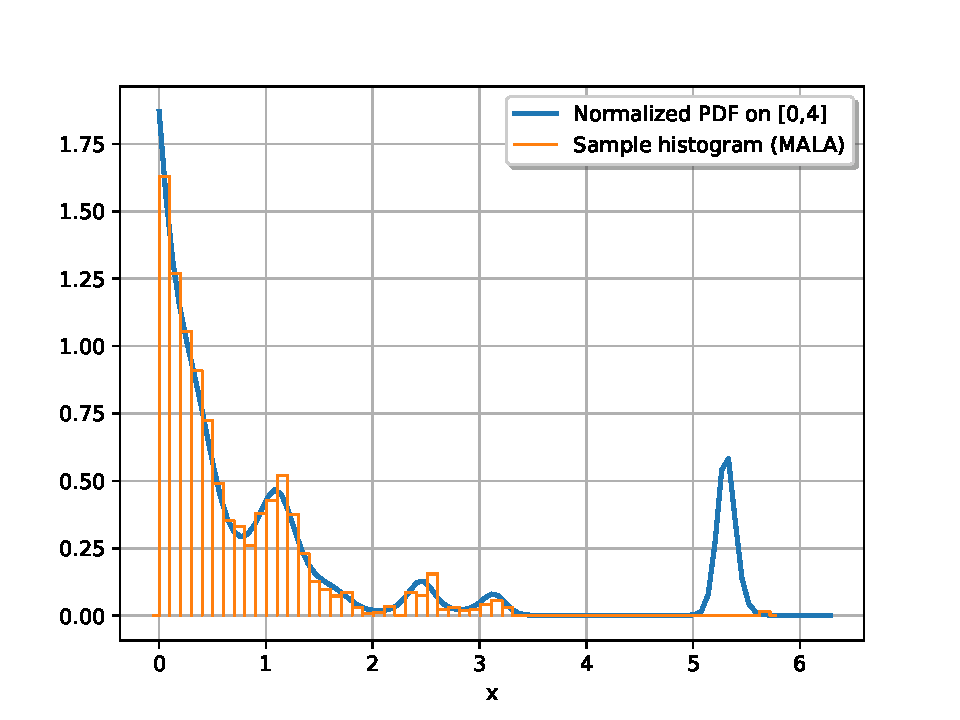
\includegraphics[width=\textwidth]{figures/MALA}
            \end{column}
            \begin{column}{0.6\textwidth}
                With $h>0$ a fixed parameter:
                \begin{equation*}
                    \proposal{q(\cdot | x)} = \proposal{\mathcal{N}}\left(x + \frac{h}{2} \frac{d}{dx} [ \log(\pi(x) ], \sqrt{h} \right)
                \end{equation*}
            \end{column}
        \end{columns}
    \end{block}
\vspace{-0.4cm}
\begin{lstlisting}
from openturns.experimental import UserDefinedMetropolisHastings
|\target{logdensity}| = ot.|Symbolic\target{Function}|('x','log(2+sin(x)^2) - (2+cos(3*x)^3+sin(2*x)^3) * x')
|\support{support}, \proposal{proposal}, initialState| = |ot.\support{Interval([0.0], [2.0 * m.pi])}, ot.\proposal{Normal()}, [2.5]|
h = 0.5
std_deviation = m.sqrt(h)

def python_link(x):
    derivative_log_density = |\target{logdensity}|.getGradient().gradient(x)[0, 0]
    mean = x[0] + h / 2 * derivative_log_density
    return [mean, std_deviation]
|\proposal{link}| = ot.PythonFunction(1, 2, python_link)

mala = UserDefinedMetropolisHastings(|\target{logdensity}|, |\support{support}|, initialState, |\proposal{proposal}|, |\proposal{link}|)
z = mala.getSample(10000)
\end{lstlisting}

\end{frame}

%%%%%%%%%%%%%%%%%%%%%%%%%%%%%%%%%%%%%%%%%%%%%%%%%%%%%%%%%%%%%%%%%%%%%%%%%%%%%
\section{Random vector Metropolis-Hastings}
\begin{frame}[containsverbatim]
    \frametitle{Random vector ``Metropolis Hastings''}

    \begin{columns}
    \begin{column}{0.5\textwidth}
        \begin{align*}
            &\observation{\boldsymbol{Y}} | \boldsymbol{\theta}, \tau \sim \likelihood{\mathcal{N}_n}(\boldsymbol{X} \boldsymbol{\theta}, \tau^{-1} \boldsymbol{I}_n + \boldsymbol{Q}^{-1}) \\
            &\boldsymbol{X} \in \mathbb{R}^{n \times p}, \boldsymbol{Q} \in \mathbb{R}^{n \times n} \mathrm{(diagonal)}\\
            &\prior{\boldsymbol{\theta} | \tau \sim 1,
            \tau \sim \tau^{-1}}
        \end{align*}
        \vspace{-1cm}
        \begin{lstlisting}
n = 10; p = 2
X = ot.Sample([[1.0]] * n)
Xcol = [[9.6], [9.5], [-16.6], [3.9], [-10.9], [7.8], [10.9], [-6.5], [15.8], [6.1]]
X.stack(Xcol)
Q = np.array([[1.4], [1.1], [4.1], [1.0], [2.9], [3.3], [1.0], [2.1], [2.9], [1.6]]) # Diagonal of Q
|\observation{Y}| = [4.9, 8.0, -16.8, 6.1, -7.1, 2.3, 10.9, -3.0, 20.2, 3.7]}

def py_link_y(x):
    theta = [x[i] for i in range(p)]
    tau = x[p]
    mean = np.dot(X, theta)
    std = np.sqrt(1.0 / tau + 1.0 / Q)
    params = np.zeros(2 * n)
    params[::2] = mean
    params[1::2] = std.ravel()
    return params
link_y = ot.PythonFunction(3,20,py_link_y)
\end{lstlisting}
    \end{column}
    \begin{column}{0.5\textwidth}
        \begin{align*}
            \boldsymbol{\theta} | \observation{\boldsymbol{Y}}, \tau \sim \proposal{\mathcal{N}_p(\boldsymbol{\mu}_n, \boldsymbol{\Sigma}_n)} \\
            \proposal{\boldsymbol{\mu}_n} = (\boldsymbol{X}^T (\boldsymbol{I}_n + \tau \boldsymbol{Q}^{-1})^{-1} \boldsymbol{X})^{-1} \\
            (\boldsymbol{X}^T (\boldsymbol{I}_n + \tau \boldsymbol{Q}^{-1})^{-1} \boldsymbol{Y}) \\
            \proposal{\boldsymbol{\Sigma}_n} = \tau^{-1} (\boldsymbol{X}^T (\boldsymbol{I}_n + \tau \boldsymbol{Q})^{-1} \boldsymbol{X})^{-1}
        \end{align*}
    \vspace{-0.8cm}
    \begin{lstlisting}
def py_link_theta(x):
    tau = x[p]
    Itilde_inv = 1.0 / (1.0 + tau / Q)
    Xtilde = Itilde_inv * X
    Sigma_n = np.linalg.inv(np.dot(Xtilde.T, X)) / tau
    mu_n = np.dot(Xtilde.T, Y)
    mu_n = tau * np.dot(Sigma_n, mu_n)
    dist = ot.Normal(|\proposal{mu\_n}|,
           ot.CovarianceMatrix(|\proposal{Sigma\_n}|)
    )
    return dist.getParameter()

|\proposal{link\_theta}| = ot.PythonFunction(3, 5, py_link_theta)

|\proposal{RVtheta}| = ot.RandomVector(|ot.\proposal{Normal(p)}|)
rvmh_theta = ot.|RandomVectorMetropolisHastings|(
    |\proposal{RVtheta}|, [1.0] * 3, [0,1], |\proposal{link\_theta}|)
\end{lstlisting}
    \end{column}
\end{columns}

\end{frame}

\begin{frame}[containsverbatim]
    \frametitle{Random vector ``Metropolis Hastings'' -- continued}
    \begin{block}{$\tau$ must be sampled the hard way, using Random walk Metropolis}
\begin{lstlisting}
proposal_tau = ot.Normal(0.0, 1e-1)
|\prior{logprior}| = |ot.Symbolic\prior{Function}|(["theta1", "theta2", "tau"], ["-log(tau)"])
support = ot.Interval([-np.inf, -np.inf, 0.0], [np.inf] * 3)}
rwmh_tau = ot.RandomWalkMetropolisHastings(|\prior{logprior}|, support, [1.0]*3, proposal_tau,[p])
rwmh_tau.setLikelihood(|ot.\likelihood{ComposedDistribution([ot.Normal()]*len(Y))}|, |\observation{[Y]}|, link_y)
\end{lstlisting}
    \end{block}
\vspace{-0.5cm}
    \begin{block}{Samplers are combined in a Gibbs algorithm}
        \centering
        
\begin{tikzpicture}[
            squarednode/.style={rectangle, draw=green!60, fill=green!5, very thick, minimum size=5mm},
            ]
            %Nodes
            \node[squarednode]      (mhxy)                     {\texttt{rwmh\_tau}};
            \node[squarednode]      (mhz)       [right=of mhxy] {\texttt{rvmh\_theta}};

            %Lines
            \draw[->] (mhxy.east) -- (mhz.west);
            \draw[->] (mhz.east) to [out=340,in=200,looseness=1.5] (mhxy.west);

        \end{tikzpicture}
\vspace{-0.3cm}
        \begin{lstlisting}
gibbs = ot.Gibbs([rwmh_tau, rvmh_theta])
sample = gibbs.getSample(10000)
sample.setDescription([r"$\theta_1$", r"$\theta_2$", r"$\tau$"])
\end{lstlisting}
    \end{block}
\vspace{-0.5cm}
\begin{figure}
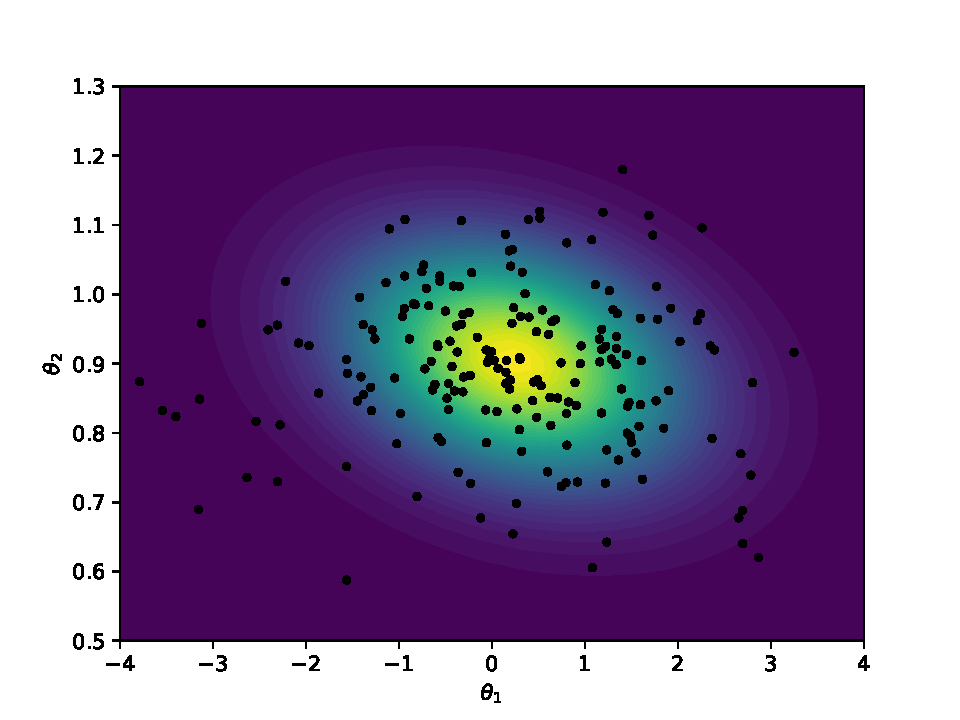
\includegraphics[width=0.32\textwidth]{figures/rvmh_blocs_theta_2_theta_1.pdf}
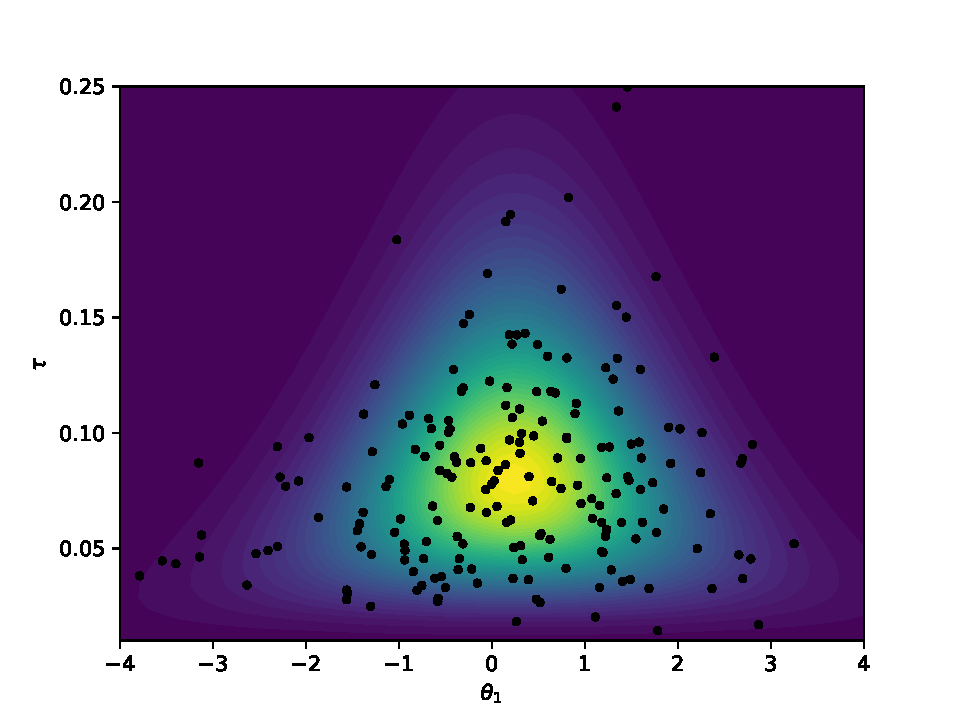
\includegraphics[width=0.32\textwidth]{figures/rvmh_blocs_tau_theta_1.pdf}
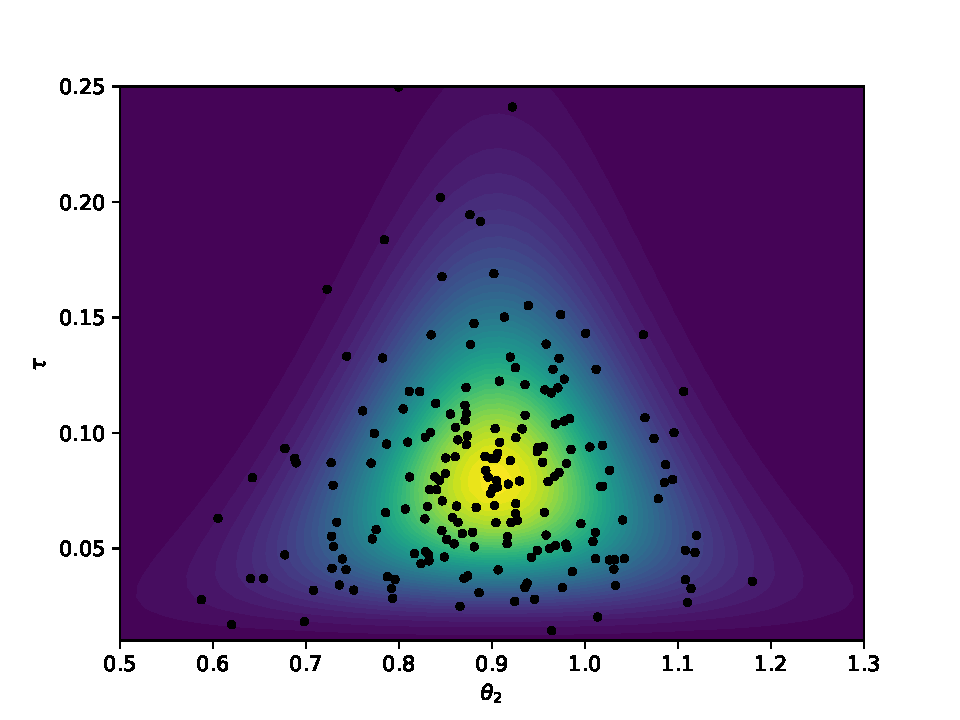
\includegraphics[width=0.32\textwidth]{figures/rvmh_blocs_tau_theta_2.pdf}
\end{figure}
\end{frame}

%%%%%%%%%%%%%%%%%%%%%%%%%%%%%%%%%%%%%%%%%%%%%%%%%%%%%%%%%%%%%%%%%%%%%%%%%%%%%
\section{Conclusion}
\begin{frame}
    \frametitle{Conclusion}
    OpenTURNS provides an MCMC sampling framework through the following classes:
    \begin{itemize}
        \item MetropolisHastings variants:
        \begin{itemize}
            \item RandomWalkMetropolisHastings
            \item IndependentMetropolisHastings
            \item UserDefinedMetropolisHastings
            \item RandomVectorMetropolisHastings
        \end{itemize}
        \item Gibbs
    \end{itemize}
    \medskip
    These classes can be freely combined to sample from nonstandard distributions
    in a ``smart'' manner. \medskip

    In a Bayesian setting, this framework allows users to create and implement
    the MCMC algorithm most suited to a particular posterior distribution.
\end{frame}
    \end{document}
